%\subsection{EW Top production veto}
\subsubsection{EW Top production veto: Tight region definition}
\label{subsec:topveto_selection}

We found that the contribution of the EW Top production is still significant in our SRs. 

As discussed in Section~\ref{sec:mc_sample_ewvvjj},
the EW Top and VVV processes are included in the signal MC samples. Since we want to enhance the VBS processes in our target phase space for the interpretation of data/MC agreement with the aQGC new physics model, we add additional selections to reduce the top contribution.

%\textcolor{red}{put here a table of the VV, VVV and top contributions in the SRs}

%\subsubsection{Loose and tight regions definition}
\label{subsec:LooseTightRegion}

We found that the resolved regions have much higher top contribution with respect to the merged ones.
For the top contribution in our signal sample, the top-quark mass can be reconstructed in the resolved SRs.
Two signal jets and the additional third jet which forms the three-jet mass, $m_{jjj}$, 
the closest to the top mass (172.76 \ GeV) are used. 
Additional third jet was chosen from all jets except for signal jets, including VBS tagging jets.
Figure \ref{fig:2leptopMass}-a shows the $m_{jjj}$ distributions for top contribution, VVV, and other components (e.g. VBS) in the EW WZjj signal sample.
We can reject the top contribution by the cut on $M_{jjj}$ at 220~\GeV.
Figure \ref{fig:2leptopMass}-b shows the data/MC comparison of the $M_{jjj}$ distribution in the \tlep \Zjets CR.
The mis-modelling in Z+jets shown in $m_{tagjj}$ was also seen in $M_{jjj}$ distribution. It is also corrected by re-weighting with $m_{tagjj}$ described in section~\ref{subsec:mjj_reweight}, though a slight slope is seen in figure \ref{fig:2leptopMass}-b, which seems to be re-weighted a little too much in this phase space.

\begin{figure}[ht]
    \begin{center}
    	\subfigure[$\text{top mass peak}$]{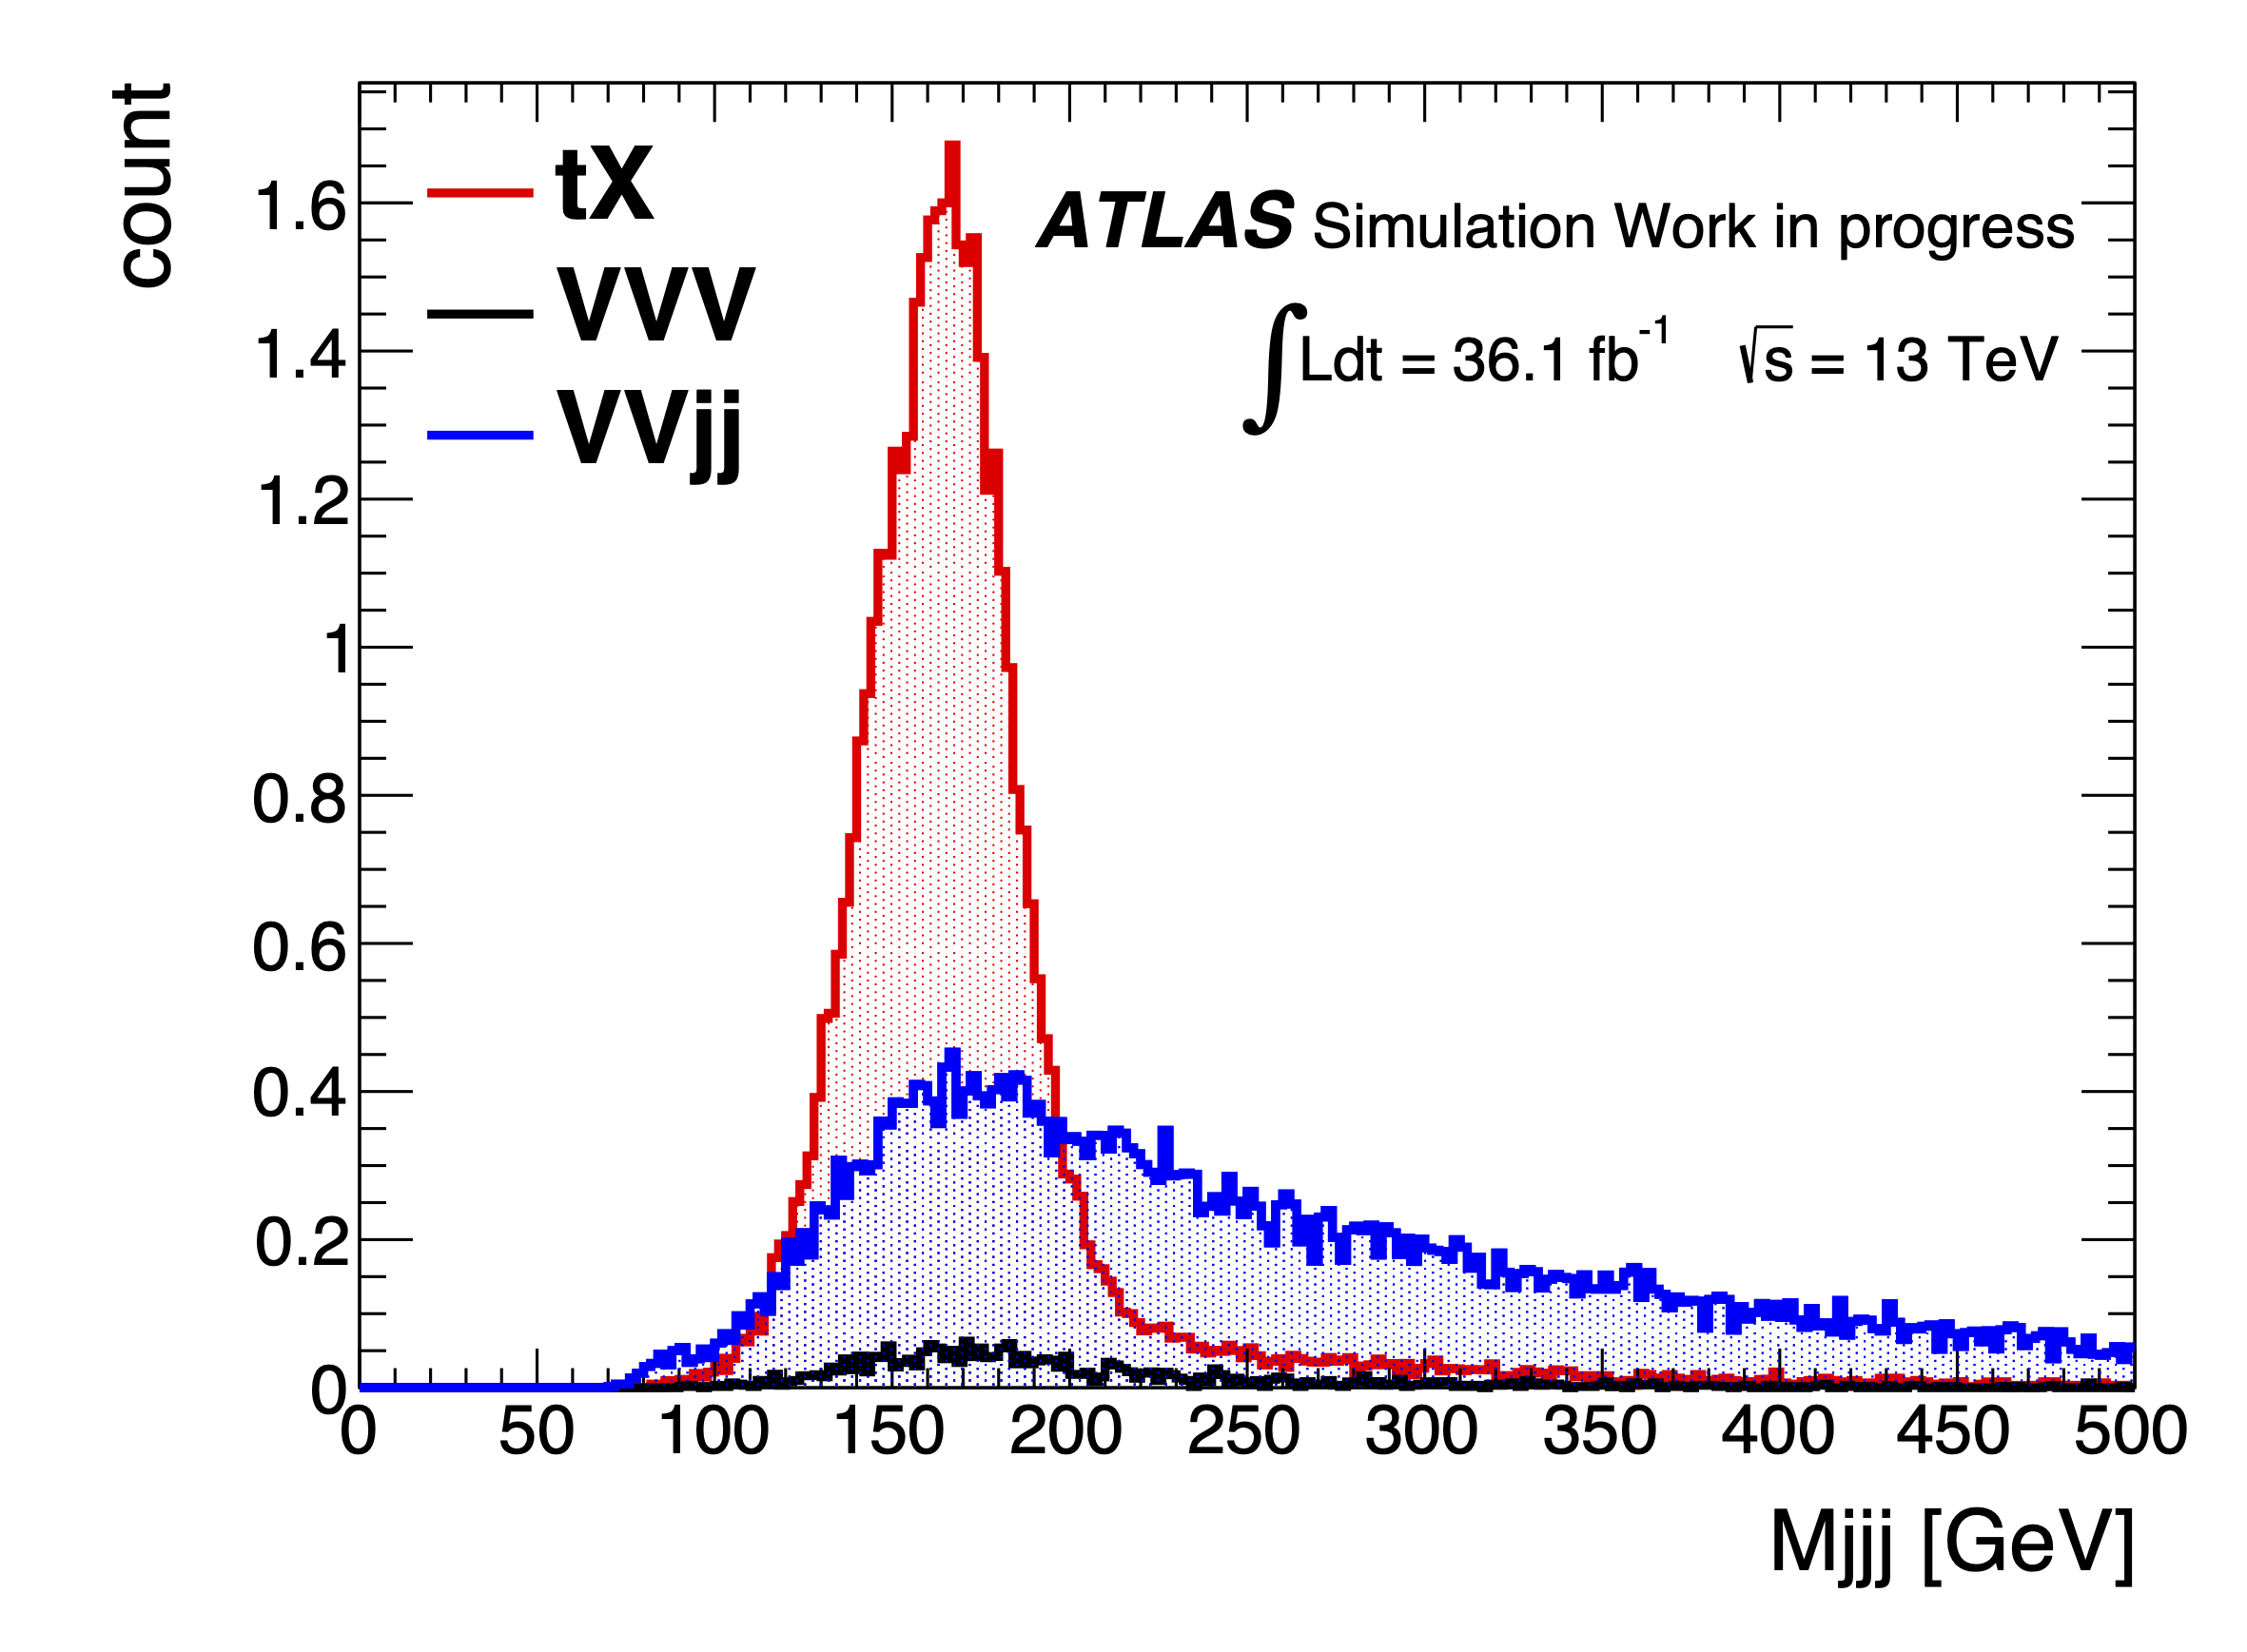
\includegraphics[width=0.4\textwidth]{figures/2lep/topMass/WZjjtopMasspeak.png}}
    	\subfigure[$\text{top mass in CRVjet}$]{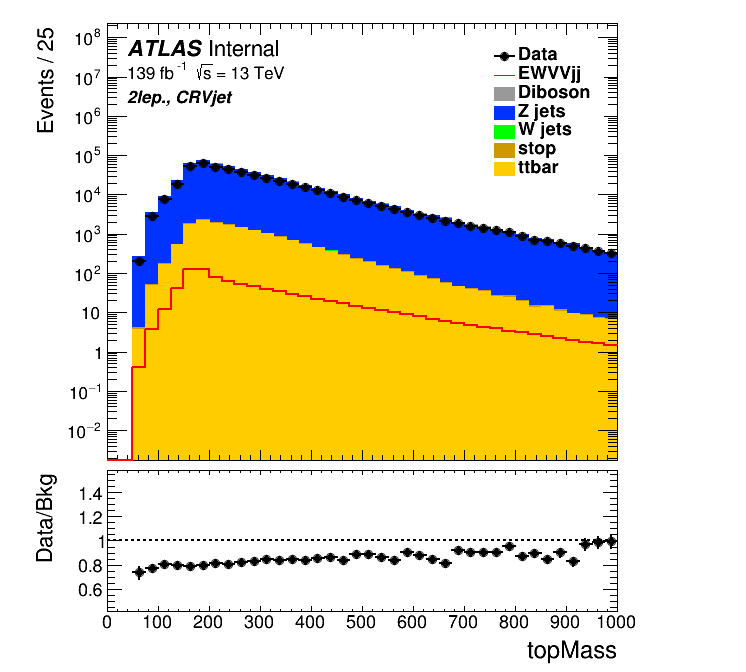
\includegraphics[width=0.4\textwidth]{figures/2lep/dataMC/C_0ptag2pjet_0ptv_CRVjet_topMass_Log.png}}
        \caption{ Mass of 3 jets in the 2-lepton channel; shapes of the signal components in the Resolved SR (a) and data to MC comparison in the \Zjets CR (b) are shown.} 
        \label{fig:2leptopMass}
    \end{center}
\end{figure}

Figure \ref{fig:0leptopMass} shows distributions for the reconstructed top mass in the \zlep channel; 
in particular, only data, signal and top background are shown to stress the most of the top background 
is rejected by this cut, while the actual data, containing the other SM background as well as the EWK signal
have higher selection efficiency in the high reconstructed top mass. 
Furthermore, the bottom pannel shows the signal to background ration that in increasing with this variable.

\begin{figure}[ht]
    \begin{center}
    	\subfigure[merged HP SR]{\includegraphics[width=0.45\textwidth]{figures/0lep/cutflow/topcheck/merged/plots/soverb_individual_SRVBS_HP_cutTopMassMer_topMassMer_cutflow.pdf}}
    	\subfigure[resolved SR]{\includegraphics[width=0.45\textwidth]{figures/0lep/cutflow/topcheck/merged/plots/soverb_individual_SRVBS_Res_cutTopMassRes_topMassRes_cutflow.pdf}}
        \caption{ Mass of $J^\text{sig}j^\text{extra}$ in merged (left) and of 3 jets $(jj)^\text{sig}j^\text{extra}$ in resolved in the \zlep channel signal regions. In particular, only the top background is shown, actual data contains also the other SM background, therefore, the data/MC is not expected to overlaid in the top pannel.} 
        \label{fig:0leptopMass}
    \end{center}
\end{figure}

The resolved SRs are divided into two sub-categories:
\begin{itemize}
  \item Loose Resolved: this is the baseline region defined in Section~\ref{subsubsec:resolved_jets_selection}, and
  \item Tight Resolved: Loose Resolved + $M_{jjj} > 220 GeV$.
\end{itemize}

\subsubsection{Signal purity in merged and resolved regimes}
\label{subsec:SignalPurity}

The contribution of the three truth components of the EW signal has been checked with previous SR definition and with new $M_{jjj}$ selections. 

Tables
\ref{tab:0leptopMassTable}-
\ref{tab:TruthTop1LepPurity}-
\ref{tab:TruthTop2LepPurity}
%shows the summary for the \olep channel; 
show the summary of purity picture applying the tight cut for the resolved and merged regimes 
respectively, in the \zlep-\olep-\tlep channels.

Based on the improvements and studies performed, the reconstructed top-mass cut is only applied in the resolved signal region to define the new tight signal region, and the merged signal regions are left as they are.

\begin{table}[ht]
    \centering
    \begin{tabular}{r|c|c|c|c}
         & \multicolumn{2}{c|}{merged HP SR} & \multicolumn{2}{c}{resolved SR}\\
         & before cut & after cut & before cut & after cut\\
         \hline
         truth top fraction in signal MC & $17\%$ & $13\%$ &$33\%$ & $9\%$ \\
         signal MC events & $94$ & $77$ & $594$ & $219$ \\
         top ($t\bar t$ + single $t$) MC events & $1786$ & $819$ & $18208$ & $1642$ \\
        \end{tabular}
        \caption{Effect of 3 jet cut in 0-lepton merged HP and resolved SR.} 
        \label{tab:0leptopMassTable}
\end{table}

\begin{table}[ht]
    \centering
	\resizebox{0.7\textwidth}{!}{
	\begin{tabular}{|c||c|c||c |c|}
    \hline
        & \shortstack{ VBS enhanced \\(resolved)} & \shortstack{non VBS enhanced \\ (resolved)} & \shortstack{VBS enhanced \\ (merged)} & \shortstack{non VBS enhanced \\ (merged)}\\
    \hline
    Truth Top       & 56.3 & 135.7 & 6.42 & 8.05 \\ 
    \hline
    Truth Triboson  & 3.85 & 9.08 & 1.72 &  2.178\\
    \hline
    Truth VBS       &  148 & 224.9 & 43.8 & 47.58\\
    \hline
    VBS purity & .711 & .608 & .843 & .823 \\
    \hline
	\end{tabular}}
    \caption{Event yields for 1lepton EW6 events in the resolved signal region and high purity merged signal region. The resolved VBS enhanced signal region is defined as events that pass the loose resolved signal region and pass $M_{jjj} >$ 220GeV. The merged VBS enhanced region is defined as events that pass the usual merged high purity signal region and pass $M_{Jj} >$ 220Gev, where $M_{Jj}$ is defined similarly to $M_{jjj}$, as the mass of the large-R jet and a third jet with total mass closest to the top mass. non-VBS enhanced regions are the old loose signal region definitions. 
%Based on the improvements shown here, the $M_{jjj}$ cut is only applied in the resolved signal region to define the new tight signal region, and the merged signal regions are left as they are. 
    }
\label{tab:TruthTop1LepPurity}
\end{table}

\begin{table}[ht]
    \centering
	\resizebox{0.70\textwidth}{!}{
	\begin{tabular}{|c||c|c|c|c|}      
        \hline
                    & SRVBS (resolved) & VBS enhanced (resolved) & SRVBS (merged) & VBS enhanced (merged) \\ \hline
    Truth Top       & 0.48             & 0.14                    & 0.14           & 0.10                  \\ \hline
    Truth VVV       & 0.03             & 0.03                    & 0.08           & 0.08                  \\ \hline
    Truth VBS       & 0.49             & 0.83                    & 0.78           & 0.82                  \\ \hline
	\end{tabular}
    }
    \caption{Fraction of event yields for 2lepton channel. Only EWWZjj events are checked here since there are no Top contributions in EWZZjj events.}
    \label{tab:TruthTop2LepPurity}
\end{table}

%\textcolor{red}{we put here the purities of the MC signal samples in the final reco regions comparing the diagram based classification for VV, VVV and EWTop}
